
	\begin{theorem}
		The application $\pi$ that we defined on the set of generators $S$ of the Coxeter system $(W,S)$, extends uniquely to an injective homomorphism $\pi\fctt{W}{S^B_T}$
	\end{theorem}
	\begin{proof}
		First of all, we need to show that the extension of $\pi$ is well defined. It was clear, due to the definition of $\pi$ on $S$ that for every $s\in S$, the application $\pi_s\in S^B_T$. Indeed, for every $t\in T$ we had that $\pi_s(t)\in T\cup \ub{T}$ and we had that $\pi_s$ defined a bijection on $T\cup \ub{T}$. Now, we need to check that its extension on all of $W$ is still well defined. We need to check 2 things. First, we need to check that $\forall w\in W$ the application $\pi_w\in S_T^B$. But, since we extended $\pi$ from $S$ to $W$ to be a group morphism, we know that $\pi_w$ is by definition the composition of $\pi_s$ for some $s\in S$ and thus is an element of $S_T^B$. Secondly, we need to check that this application $\pi_w$ does not depend on the writing of $w\in W$. To this aim, let us take $t\in T$ and let $w=s_1s_2..s_k$ for some $s_i\in S$ (this is the form of every element of $W$ since $s_i=s_i^{-1}$ for all $i$). Since, we want $\pi$ to be a homomorphism, we have that :
		\begin{equation}\label{equation donnant la form explicite de pi}
		\begin{split}
		\pi_w(t)\qq&=\qq \pi_{s_1}\circ\pi_{s_2}\circ ... \circ \pi_{s_k}(t)\\
		&=\qq \pi_{s_1}\circ\pi_{s_2}\circ ... \circ \pi_{s_{k-1}}(\pm s_kts_k)\q\q\\
		& \q\q (\mbox{with }-\mbox{ iff }s_kts_k=s_k\iff t=s_k)\\
		&=\qq \pi_{s_1}\circ\pi_{s_2}\circ ... \circ \pi_{s_{k-2}}(\pm\pm s_{k-1}s_kts_ks_{k-1})\q\q\\
		& \q\q(\mbox{with }-\mbox{ iff }s_{k-1}s_kts_ks_{k-1}=s_{k-1}\iff t=s_ks_{k-1}s_k)\\
		&=\qq \pi_{s_1}\circ\pi_{s_2}\circ ... \circ \pi_{s_{k-3}}(\pm\pm\pm s_{k-2}s_{k-1}s_kts_ks_{k-1}s_{k-2})\q\q \\
		&\q\q (\mbox{with }-\mbox{ iff }s_{k-1}s_kts_ks_{k-1}=s_{k-1}s_{k-2}\iff t=s_ks_{k-1}s_{k-2}s_{k-1}s_k)\\
		&=\q\q \q\vdots\q\q \q\vdots\q\q \q\vdots\q\q \q\vdots\q\q \q\vdots\q\q \q\vdots\q\q \q\vdots\q\q \q\vdots\q\q \q\vdots\\
		&=\qq \pm\pm \dots \pm s_1s_2...s_kts_ks_{k-1}... s_1\q\q\\
		& \q\q (\mbox{with }-\mbox{ iff }s_1...s_{k-1}s_kts_ks_{k-1}...s_1=s_{1}\iff t=s_k...s_2s_1s_2...s_k)\\
		&=\mbox{sgn}_w(t)\qq wtw^{-1}
		\end{split}
		\end{equation}
		where the function $\mbox{sgn}_w(t)$ is a sign function counting the number of times we have an index $l\in \{1,2,...k\}$ such that $t=s_k...s_{l-1}s_l s_{l-1}...s_k$. Namely :
		\begin{equation}
		 \mbox{sgn}_w(t)\qq=\qq (-1)^{\# \{1\leq l\leq k\qq :\qq t=s_k...s_{l-1}s_l s_{l-1}...s_k\}}
		\end{equation}
		As we will show just after this sign function does not depend of the writing of $w\in W$ in the Coxeter system $(W,S)$.

		But first, let us get some intuition about what this sign function is counting with a visual representation that we have seen before in the chapter: wiring diagrams. In figure \ref{fig:wiring_sign} you can find an example for $S_n$.
		\begin{figure}

		  \begin {center}
		  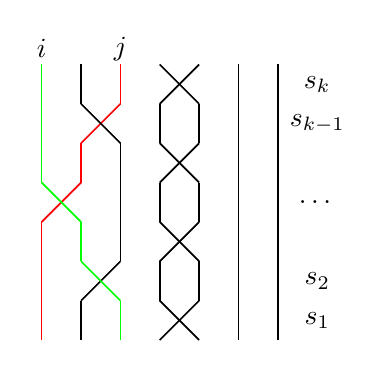
\begin{tikzpicture}

				\def\xa{0}
				\def\xb{0.5}
				\def\xc{1}
				\def\xd{1.5}
				\def\xe{2}
				\def\xf{2.5}
				\def\xg{3}

				%first level
				\draw[semithick, color=red] (\xa,0) -- (\xa,0.5);
				\draw[semithick] (\xb,0) -- (\xb,0.5);
				\draw[semithick, color=green] (\xc,0) -- (\xc,0.5);
				\draw[semithick] (\xd,0) -- (\xe,0.5);
				\draw[semithick] (\xe,0) -- (\xd,0.5);
				\draw[semithick] (\xf,0) -- (\xf,0.5);
				\draw[semithick] (\xg,0) -- (\xg,0.5);

				%second level
				\draw[semithick, color=red] (\xa,0.5) -- (\xa,1);
				\draw[semithick] (\xb,0.5) -- (\xc,1);
				\draw[semithick, color=green] (\xc,0.5) -- (\xb,1);
				\draw[semithick] (\xd,0.5) -- (\xd,1);
				\draw[semithick] (\xe,0.5) -- (\xe,1);
				\draw[semithick] (\xf,0.5) -- (\xf,1);
				\draw[semithick] (\xg,0.5) -- (\xg,1);

				%third level
				\draw[semithick, color=red] (\xa,1) -- (\xa,1.5);
				\draw[semithick, color=green] (\xb,1) -- (\xb,1.5);
				\draw[semithick] (\xc,1) -- (\xc,1.5);
				\draw[semithick] (\xd,1) -- (\xe,1.5);
				\draw[semithick] (\xe,1) -- (\xd,1.5);
				\draw[semithick] (\xf,1) -- (\xf,1.5);
				\draw[semithick] (\xg,1) -- (\xg,1.5);

				%fourth level
				\draw[semithick, color=red] (\xa,1.5) -- (\xb,2);
				\draw[semithick, color=green] (\xb,1.5) -- (\xa,2);
				\draw[semithick] (\xc,1.5) -- (\xc,2);
				\draw[semithick] (\xd,1.5) -- (\xd,2);
				\draw[semithick] (\xe,1.5) -- (\xe,2);
				\draw[semithick] (\xf,1.5) -- (\xf,2);
				\draw[semithick] (\xg,1.5) -- (\xg,2);

				%fifth level
				\draw[semithick, color=green] (\xa,2) -- (\xa,2.5);
				\draw[semithick, color=red] (\xb,2) -- (\xb,2.5);
				\draw[semithick] (\xc,2) -- (\xc,2.5);
				\draw[semithick] (\xd,2) -- (\xe,2.5);
				\draw[semithick] (\xe,2) -- (\xd,2.5);
				\draw[semithick] (\xf,2) -- (\xf,2.5);
				\draw[semithick] (\xg,2) -- (\xg,2.5);

				%sixth level
				\draw[semithick, color=green] (\xa,2.5) -- (\xa,3);
				\draw[semithick, color=red] (\xb,2.5) -- (\xc,3);
				\draw[semithick] (\xc,2.5) -- (\xb,3);
				\draw[semithick] (\xd,2.5) -- (\xd,3);
				\draw[semithick] (\xe,2.5) -- (\xe,3);
				\draw[semithick] (\xf,2.5) -- (\xf,3);
				\draw[semithick] (\xg,2.5) -- (\xg,3);

				%seventh level
				\draw[semithick, color=green] (\xa,3) -- (\xa,3.5);
				\draw[semithick] (\xb,3) -- (\xb,3.5);
				\draw[semithick, color=red] (\xc,3) -- (\xc,3.5);
				\draw[semithick] (\xd,3) -- (\xe,3.5);
				\draw[semithick] (\xe,3) -- (\xd,3.5);
				\draw[semithick] (\xf,3) -- (\xf,3.5);
				\draw[semithick] (\xg,3) -- (\xg,3.5);

				\draw (\xa,3.7) node {$i$};
		   	\draw (\xc,3.7) node {$j$};

				\draw (\xg+0.5,3.25) node {$s_k$};
				\draw (\xg+0.5,2.75) node {$s_{k-1}$};
				\draw (\xg+0.5,1.75) node {\ldots};
				\draw (\xg+0.5,0.75) node {$s_2$};
				\draw (\xg+0.5,0.25) node {$s_1$};

		  \end{tikzpicture}
		  \caption{ A wiring diagram for a word $w \in W$ of the coxeter group $S_n$. You can see that $sgn_w(t)$ with $t = (i,j)$ equals 1 because there is only one crossing between the wires that begin at $i$ and $j$.}
		  \end{center}
		\label{fig:wiring_sign}
		\end{figure}



		We are now going to use equation \ref{equation donnant la form explicite de pi} to prove that $\pi$ is a well defined homomorphism which is equivalent to show that the sign function does not depend on the writing of $w\in W$ in the Coxeter system $(W,S)$. It suffices to show that all the relations we had in $(W,S)$ are satisfied by their image in $S^B_T$. I.e. let us take $s,s'\in S$, we want to show that :
		\begin{equation}\label{equation provant que les relations sont preserves par pi}
		(\pi_s\circ \pi_{s'})^{m(s,s')}\qq=\qq \mbox{Id}_{S^B_T}
		\end{equation}
		Since $(ss')^{-1}=s's$, equation \ref{equation donnant la form explicite de pi} gives for all $t\in T$ :
		\begin{equation}
		(\pi_s\circ \pi_{s'})^{m(s,s')}(t)\qq=\qq \pm\qq (ss')^{m(s,s')}t(s's)^{m(s,s')}\qq=\qq \pm \qq et e\qq=\qq\pm \qq  t
		\end{equation}
		But the sign must be $+$ as here, $w=(ss')^{m(s,s')}$ and therefore we look at :
		\begin{equation}
		{\# \{1\leq l\leq m(s,s') \qq :\qq t=\underset{2l-1 \mbox{ characters}}{\underbrace{s'ss'...s'ss'}}\}}
		\end{equation}
		Which must be even. Indeed, if for some $l\leq m(s,s')/2$ we have :
		\begin{itemize}
			\item if $ m(s,s')$ is even :
			\begin{equation}
			t\qq=\qq \underset{2l-1 \mbox{ characters}}{\underbrace{s'ss'...s'ss'}}\qq=\qq\underset{2l-1 + m(s,s') \mbox{ characters}}{\underbrace{s'ss'...s'ss'}}\qq=\qq \underset{2(l+m(s,s')/2)-1 \mbox{ characters}}{\underbrace{s'ss'...s'ss'}}
			\end{equation}
			\item  if $ m(s,s')$ is odd :
			\begin{equation}
			t\qq=\qq \underset{2l-1 \mbox{ characters}}{\underbrace{s'ss'...s'ss'}}\qq=\qq\underset{2l-1 +m(s,s') \mbox{ characters}}{\underbrace{s'ss'...s'ss'}}\qq=\qq \underset{2((m(s,s')-1)/2+l)+1 \mbox{ characters}}{\underbrace{s'ss'...s'ss'}}
			\end{equation}
		\end{itemize}
	This shows that if one index is counted below $m(s,s')/2$ then there exists an other index counted strictly upper than $m(s,s')/2$ and vis versa. Thus the set must be even and the sign must be $+$. Therefore, equation \eqref{equation provant que les relations sont preserves par pi}, is proved and we $\pi$ is a well defined morphism.

	It remains to show that the extension of $\pi$ is injective. Let $u,v\in W$ be such that $\pi_u=\pi_v$ then, we have that :
	\begin{equation}
	\pi_{uv^{-1}}\qq=\qq \pi_u\circ \pi_{v^{-1}}\qq=\qq \mbox{Id}_{S_T^B}\qq=\qq  \pi_e
	\end{equation}
	Thus, we just need to show that if $w\in W$ is such that $\pi_w=\pi_e$ then $w=e$ to prove the injectivity of $\pi$. Now, let us take $w\in W$ such that $\pi_w=\pi_e$ and let us suppose absurdly that $w\not=e$ then, there exists $k\geq 1$ such that $w=s_1...s_k$ is the shorter way possible to write $w\in W$ then (meaning that $k$ is the smallest possible) :
	\begin{equation}\label{equation pour la contradiction par signe de sk}
	\begin{split}
		s_k\qq=\qq\pi_e(s_k)\qq&=\qq \pi_w(s_k)\qq =\qq\mbox{sgn}_w(s_k)\qq s_1...s_{k-1}s_ks_ks_ks_{k-1}...s_1\qq\\
		&=\qq\mbox{sgn}_w(s_k)\qq s_1...s_{k-1}s_ks_{k-1}...s_1
	\end{split}
	\end{equation}
	But $\mbox{sgn}_w(s_k)=-1$ because :
	\begin{equation}
	\{1\leq l\leq k\qq :\qq t=s_k...s_{l-1}s_l s_{l-1}...s_k\}\qq=\qq \{k\}
	\end{equation}
	Indeed, for $l=k$ we have $s_k=s_k$. But if $l\not=k$ and if we had :
	\begin{equation}
	s_k=\qq s_k..s_l..s_k
	\end{equation}
	Then we would have :
	\begin{equation}
	s_{l-1}...s_ks_k\qq=\qq s_l...s_k
	\end{equation}
	Therefore, we would have a contradiction with the minimality of $k$ since :
	\begin{equation}
	\begin{split}
	w&=s_1...s_ls_{l-1}s_l...s_k\qq\\
	&=\qq s_1...s_{l-1}s_{l-1}...s_ks_k\qq\\
	&=\qq s_1..s_{l-2}s_{l+1}...s_{k-1}\qq\\
	&=\qq s_1...s_{l-2}s_{l+11}...s_{k-1}
	\end{split}
	\end{equation}
	which is a shorter way to write $w$. Therefore, we have that $\mbox{sgn}_w(s_k)=-1$ and thus equation \ref{equation pour la contradiction par signe de sk} gives :
	\begin{equation}
			s_k\qq=\qq -\qq  s_1...s_{k-1}s_ks_{k-1}...s_1
	\end{equation}
	which is a contradiction due to the presence of a sign.\qed
	\end{proof}


	We are now going to define the notions of \tg{parity} and \tg{length} of an element in a Coxeter group.
	\begin{definition}
		Let $(W,S)$ be a Coxeter system, and let $w\in W$, then we say that $w=s_1...s_k$ $(s_l\in S)$ is :
		\begin{itemize}
			\item \tg{even} when $k$ is even.
			\item \tg{odd} when $k$ is odd.
		\end{itemize}
	This is what we call the \tg{parity} of $w\in W$.
	\end{definition}
\begin{remark}
	As all the relations of a Coxeter group involve a pair number of $s\in S$ we see that the parity of an element $w\in W$ doesn't depend on its writing in $W$.
\end{remark}
The set of even elements of a Coxeter system $(W,S)$ is a subgroup of $W$ called the \tg{alternating} subgroup.
\begin{remark}
	When $S_n$ is seen as a Coxeter group with $S=\{s_1...s_{n-1}\}$ and the Coxeter matrix $m(s_i,s_{i+1})=3$ and $m(s,s')=2$ for every other couple $(s,s')\not=(s,s)$ see that the two notions of alternating group coincide.
\end{remark}
\begin{definition}
	Let $(W,S)$ be a Coxeter system, the \tg{length} $l(w)$ of an element $w\in W$ is defined as the smallest integer $k\in \N$ such that there exists $s_1,...,s_k\in S$ with $w=s_1...s_k$.
\end{definition}
The purpose of what follows is to prove the following theorem :
\begin{theorem}\label{theorem sur le calcul des longueurs}
	Let $(W,S)$ be a Coxeter system, and let $w\in W$ then :
	\begin{equation}
	l(w)\qq=\qq \#\{t\in T\qq :\qq \mbox{sgn}_{w^{-1}}(t)=-1\}
	\end{equation}
\end{theorem}
\begin{example}
	In the case where $W=S_n$ with the common representation, $l(w)$ is exactly the number of inversions of $w^{-1}$ which is exactly the same as the number of inversions of $w$ itself.
\end{example}
Before proving this theorem, we focus our attention on some lemma :
\begin{lemma}\label{le lemme de la longueur de tw}
	Let $(W,S)$ be a Coxeter system and let $w\in W$, $t\in T$ then :
	\begin{equation}
	\mbox{sgn}_{w^{-1}}(t)=-1\q \iff \q l(tw)\qq<\qq l(w)
	\end{equation}
\end{lemma}
\begin{proof}
	Let's suppose that $\mbox{sgn}_{w^{-1}}(t)=-1$ and let $w=s_1...s_k$ with $k=l(w)$ then $w^{-1}=s_k...s_1$. We know that there must exist some $1\leq l\leq k$ such that $t=s_1...s_l..s_1$ but then :
	\begin{equation}
	\begin{split}
	tw\qq&=\qq s_1s_2...s_l...s_1\qq q_1s_2...s_ls_{l+1}...s_k\\
	&=\qq s_1s_2...s_{l-1}s_{l+1}...s_k\\
	&=\qq s_1s_2...\hat{s_l}...s_k
	\end{split}
	\end{equation}
	from which we conclude that $l(tw)\leq k-1\qq <\qq k=l(w)$ and the first implication is proven.\\
	Conversely, let's suppose that $l(tw)<l(w)$ then, as $tt=e$ we have that :
	\begin{equation}
	l(tw)\qq <\qq l(ttw)\qq \Rightarrow l(ttw)\not<l(tw)
	\end{equation}
	Therefore, the first implication that we already proved, gives us by taking $\tilde{w=tw}$ that :
	\begin{equation}
	\mbox{sgn}_{w^{-1}t}(t)=+1
	\end{equation}
	Thus,
	\begin{equation}
	\pi_{(tw)^{-1}}(t)\qq=\qq +1 \qq (tw)^{-1}\qq t\qq(tw)\qq=\qq w^{-1}tw
	\end{equation}
	But, by the fact that $\pi$ is a morphism we have that :
	\begin{equation}\label{pi est un homo}
	\pi_{(tw)^{-1}}\qq=\qq\pi_{w^{-1}t}\qq=\qq =\pi_{w^{-1}}\circ\pi_t
	\end{equation}
	Now let's remark that $\forall t\in T$ we have that :
	\begin{equation}
	\pi_t(t)\qq=\qq \mbox{sgn}_t(t)\qq ttt\qq=\qq -t
	\end{equation}
	Indeed, let's write $t=s_1...s_kss_k...s_1$ for a $k$ that is minimal. Then it is clear that :
	\begin{equation}\label{le signe de t de t}
	\{1\leq l\leq 2k+1\qq :\qq t=s_1...s_{l-1}s_l s_{l-1}...s_1\}\qq=\qq \{k+1\}
	\end{equation}
	as by the minimality, it can't be true for $l\leq k$ that $t=s_1...s_{l-1}s_l s_{l-1}...s_1$ and as if it is true for some $l= k+1+l'$ with $l'>0$ we have that
	\begin{equation}
	t\qq=\qq s_1s_2...s_kss_k...s_{k-l'+1}s_{k-l'}s_{k-l'+1}...s_kss_k...s_2s_1
	\end{equation}
	Therefore, by multiplying both sides by $s_1s_2...s_ks$ from the right and by $ss_k...s_2s_1$ from the left, we obtain that :
	\begin{equation}
	s\qq=\qq s_k...s_{k-l'+1}s_{k-l'}s_{k-l'+1}...s_k
	\end{equation}
	Therefore, by replacing $s$ in $t$ we have that :
	\begin{equation}
	t\qq=\qq s_1...s_kss_k...s_1\qq=\qq s_1...s_ks_k...s_{k-l'+1}s_{k-l'}s_{k-l'+1}...s_ks_k...s_1\qq=\qq s_1...s_{k-l'}...s_1
	\end{equation}
	which again contradicts the minimality of $k$. Therefore, the equality \eqref{le signe de t de t} is verified and we have that :
	\begin{equation}
	\pi_t(t)\qq=\qq -t
	\end{equation}
	And by computing equality \eqref{pi est un homo} on $t$ we obtain that :
	\begin{equation}
	\begin{split}
	\pi_{(tw)^{-1}}(t)\qq&=\qq \pi_{w^{-1}}\pi_t(t)\qq\\
	&=\qq \pi_{w^{-1}}(-t)\qq\\
	&=\qq -\qq \pi_{w^{-1}}(t)\\
	&=\qq -\mbox{sgn}_{w^{-1}}(t)\qq w^{-1}tw
	\end{split}
	\end{equation}
	And we finally conclude that $\mbox{sgn}_{w^{-1}}(t)=-1$.\qed
\end{proof}

As a Corollary we have the following lemma :
\begin{lemma}[Exchange property]
Let $(W,S)$ be a Coxeter system and let $w=s_1s-2...s_k\in W$ and $t\in T$, then, if $l(tw)<l(w)$ then, there exists some $1\leq l\leq k$ such that :
	\begin{equation}
	tw\qq=\qq s_1s_2...\hat{s_l}... s_k
	\end{equation}
\end{lemma}
\begin{proof}
	By the previous lemma, we know that $\mbox{sgn}_{w^{-1}}t\qq=\qq -1$. Therefore, we know there exists a $1\leq l\leq k$ such that $tw\qq=\qq s_1s_2...\hat{s_l}... s_k$.\qed
\end{proof}
\begin{lemma}
	Let $(W,S)$ be a Coxeter system and let $w=s_1s_2...s_k\in W$, with $k=l(w)$ and let's take $t\in T$. Then, the following are equivalent :
	\begin{enumerate}
		\item $l(tw)<l(w)$
		\item $tw\qq=\qq s_1...\hat{s_l}...s_1$ for some $1\leq l\leq k$
		\item $t=s_1...s_l...s_1$ for some $1\leq l\leq k$
	\end{enumerate}
Moreover, such an $l$ is uniquely determined.
\end{lemma}
\begin{proof}
	By Lemma \ref{le lemme de la longueur de tw} we already know that $(1)$ implies $(2)$. Furthermore, the equivalence between $(2)$ and $(3)$ is a tautology. Let us prove that $(2)$ implies $(1)$. Indeed, if $tw\qq=\qq s_1...\hat{s_l}...s_1$ for some $1\leq l\leq k$ then :
	\begin{equation}
	l(tw)\qq \leq \qq k+1\qq <\qq k \qq=\qq l(w)
	\end{equation}
	which is $(1)$. It remains to show that this $l$ appearing in property $(2)$ and $(3)$ is unique under the hypothesis that $k=l(w)$. Let us define $t_i=s_1s_2...s_i...s_1$ for all $1\leq i\leq k$. Then, we want to show that  $t_i\not=t_j$ for every $i\not=j$. Let's reason by absurd and suppose the contrary. Therefore, there exists $i<j$ such that $t_i=t_j$. Then,
	\begin{equation}
	\begin{split}
	w\qq&=\qq t_it_j\qq w\\
	&=\qq t_is_1...\hat{s_j}...s_k\\
	&=\qq s_1...\hat{s_i}...\hat{s_j}...s_k
	\end{split}
	\end{equation}
	as $i$ was less than $j$. But this is a contradiction with the exchange property applied for $t=t_it_j$. Therefore we needed that $t_i\not=t_j$ for every $i\not=j$. In particular $l$ must be unique.
	\qed
\end{proof}
With all those lemma, we are now ready to prove theorem \ref{theorem sur le calcul des longueurs}.
\begin{proof}
	Let $w=s_1s_2...s_k$ with $k=l(w)$, then $w^{-1}=s_k...s_1$ and due to the previous lemma, we know that :
	\begin{equation}
	\begin{split}
		\#\{t\in T\qq :\qq \mbox{sgn}_{w^{-1}}(t)=-1\}\qq\q\q\q\q\q\q\q \\
		=\qq \# \{t\in T\qq:\qq t=s_1...s_i...s_k\qq \mbox{for some }1\leq l\leq k\}\qq=\qq k\qq =l(w)
	\end{split}
	\end{equation}
	as every of the $t_i=s_1...s_i...s_1$ are different from each other. \qed
\end{proof}


The following theorem describes the writing reduction of a world in a Coxeter group when it's not written in one of its minimal writings.
\begin{theorem}[Deletion property]
Let $(W,S)$ be a Coxeter system and let $w=s_1s_2...s_k$ for some $k$ with $l(w)<k$ then there exists two different indices $1\leq i<j\leq k$ such that :
	\begin{equation}
	w\qq=\qq s_1...\hat{s_i}...\hat{s_j}...s_k
	\end{equation}
\end{theorem}
A consequence is the following proposition :
\begin{proposition}
	Let $(W,S)$ be a Coxeter system and let $w=s_1...s_k$ for some $s_i\in S$ then, if $l(w)<k$ there exists a sub-word $s_{i_1}...s_{i_{l(w)}}$ of $s_1...s_k$ such that $w=s_{i_1}...s_{i_{l(w)}}$.
\end{proposition}
This proposition is used in the following :
\begin{proposition}
	Let $(W,S)$ be a Coxeter system, and let's suppose that $w=s_1s_2...s_k=s_1's_2'...s_k'$ for some $s_i,s_i'\in S$ with $k=l(w) $. Then, \begin{equation}
	\{s_1,s_2...s_k\}\qq=\qq \{s_1',s_2'...s'_k\}
	\end{equation}
\end{proposition}
\begin{remark}
	To be precise, the upper equality is an equality of sets an not of multi-sets. Indeed, as a simple example that the multi-sets can be different, we take the Coxeter group $S_3$ and the permutation $(2,3)(1,2)(2,3)=(1,3)=(1,2)(2,3)(1,2)$. Therefore, we have the multi-sets :
	\begin{equation}
	\{(2,3),(1,2),(2,3)\}\q \mbox{and}\q \{(1,2),(2,3),(1,2)\}
	\end{equation}
\end{remark}
\begin{proof}
	Suppose that the two sets are not equal. Therefore, there exists an $1\leq i\leq k$ minimal such that $s_i\not\in  \{s_1',s_2'...s'_k\}$. Furthermore, by lemma \ref{les equivalences pour tw}\textbf{Bad reference here} we know that :
	\begin{equation}
	\begin{split}
	\{s_1'...s_j'...s_1':j=1,2,...,k\}\qq&=\qq \{t\in T\qq:\qq l(tw)<l(w)\}\qq\\
	&=\qq \{s_1...s_j...s_1:j=1,2,...,k\}
	\end{split}
	\end{equation}
	As those sets are equal, there must be an index $1\leq j\leq k$ such that for our previous $i$ we have :
	\begin{equation}
	s_1...s_i...s_1\qq=\qq s_1'...s_j'...s_1'
	\end{equation}
	In particular, by previous proposition, there exists a sub-word of the right hand side which is of size $1$ and which is equal to $s_i\in W$. Therefore, either $s_i$ is one of the previous $s_1...s_{i-1}$ which would be a contradiction with the minimality of $i$, or $s_i$ is one of the $s_1',...,s_j'$ which is a contradiction with our choice of $i$. Therefore, the two sets must be the same.
\end{proof}
